%Nous avons vu que les courbes~\ref{King_Modele-test} peuvent être divisées en deux parties : l'une, caractérisée par une densité constante, constituant un cœur, et l'autre constituant un halo.
%Nous allons donc considérer un amas d'étoile composé d'un cœur dense et d'un halo.
%Le halo a peu de gravité et se comporte comme un gaz parfait.
%Le comportement observé dans notre étude est résumé sur le schéma~\ref{schema-effondrement} :
%
	\begin{figure}[ht!]
		\begin{minipage}[b]{0.20\linewidth}
			\begin{center}
				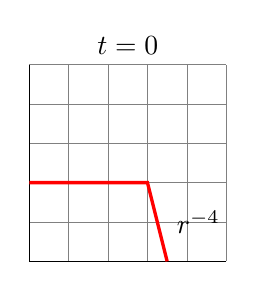
\begin{tikzpicture}
%					Tracé de la grille :
					\draw[step=.5cm,gray,very thin] (0,0) grid (2.5,2.5);
%					Tracé des axes :
					\draw (0,0) -- (0,2.5);
					\draw (0,0) -- (2.5,0);
%					Tracé du graphe :
					\draw[red,very thick] (0,1.0) -- (1.5,1.0) -- (1.75,0);
%					\draw[red,very thick] (1.5,1.0) -- (1.75,0);
					\draw (1.75,0.5) node[right]{$r^{-4}$};
					\draw (1.25,2.5) node[above]{$t = 0$};
				\end{tikzpicture}
			\end{center}
		\end{minipage}\hfill
		\begin{minipage}[b]{0.20\linewidth}
			\begin{center}
				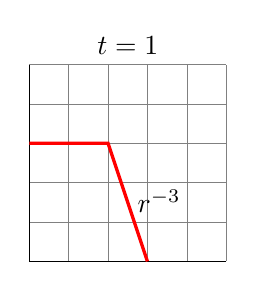
\begin{tikzpicture}
%					Tracé de la grille :
					\draw[step=.5cm,gray,very thin] (0,0) grid (2.5,2.5);
%					Tracé des axes :
					\draw (0,0) -- (0,2.5);
					\draw (0,0) -- (2.5,0);
%					Tracé du graphe :
					\draw[red,very thick] (0,1.5) -- (1,1.5) -- (1.5,0);
%					\draw[red,very thick] (1,1.5) -- (1.5,0);
					\draw (1.25,0.5) node[above right]{$r^{-3}$};
					\draw (1.25,2.5) node[above]{$t = 1$};
				\end{tikzpicture}
			\end{center}
		\end{minipage}\hfill
		\begin{minipage}[b]{0.24\linewidth}
			\begin{center}
				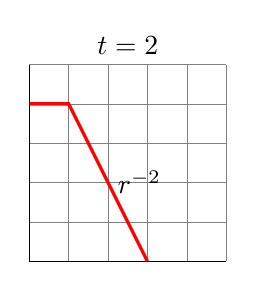
\begin{tikzpicture}
%					Tracé de la grille :
					\draw[step=.5cm,gray,very thin] (0,0) grid (2.5,2.5);
%					Tracé des axes :
					\draw (0,0) -- (0,2.5);
					\draw (0,0) -- (2.5,0);
%					Tracé du graphe :
					\draw[red,very thick] (0,2) -- (0.5,2) -- (1.5,0);
%					\draw[red,very thick] (0.5,2) -- (1.5,0);
					\draw (1,1) node[right]{$r^{-2}$};
					\draw (1.25,2.5) node[above]{$t = 2$};
				\end{tikzpicture}
			\end{center}
		\end{minipage}\hfill
		\begin{minipage}[b]{0.20\linewidth}
			\begin{center}
				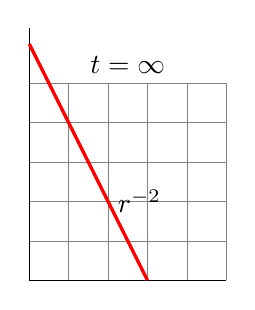
\begin{tikzpicture}
%					Tracé de la grille :
					\draw[step=.5cm,gray,very thin] (0,0) grid (2.5,2.5);
%					Tracé des axes :
					\draw (0,0) -- (0,3.2);
					\draw (0,0) -- (2.5,0);
%					Tracé du graphe :
					\draw[red,very thick] (0,3) -- (1.5,0);
					\draw (1,1) node[right]{$r^{-2}$};
					\draw (1.25,2.5) node[above]{$t = \infty$};
				\end{tikzpicture}
			\end{center}
		\end{minipage}
		\caption{Schéma d'évolution dynamique d'un amas globulaire.\label{schema-effondrement}}
	\end{figure}


%(~la pente $-4$ avec laquelle commence le schéma vient des résultats de simulations numériques~).
%La question à laquelle nous souhaitons répondre est : comment expliquer qu'un amas évolu en augmentant la densité de son cœur et en diminuant la pente avec laquelle le halo décroit ?

%Pour commencer, un amas doit, lorsqu'il est à l'équilibre, suivre un modèle de \textsc{King} ou de sphère isotherme en boîte. Par conséquent, notre amas est au Viriel.
%De plus, le cœur est un systéme auto-gravitant décrit par la thermodynamique. L'un de ses propriétés thermodynamique les plus importante à ce niveau est sa capacité calorifique. En effet :
%Nous cherchons à concentrer la matière dans le cœur de l'amas, et donc y rajouter de la matière à partir du halo (~qui va se diluer~).
%Pour faire diminuer le rayon de l'orbite d'un astre, il faut augmenter sa vitesse~\footnote{rappel : $v^2 = K\left(\frac{2}{r} - \frac{1}{a}\right)$ avec $K = G\left(M+m\right)$
%pour des interactions à deux corps}, et donc sa température. En se rappelant les résultats sur les diagrammes d'énergie de la sphère isotherme, nous nous rendons bien compte que, si la température
%augmente trop, le cœur va passer dans la zone instable, et s'effondrer.

%Le processus pour faire augmenter la température auquel nous nous attèlerons dans la suite est assez simple : l'amas évolue dans le potentiel galactique ; il va en traverser le disque de façon périodique.
%Moments pendant lesquels il va se faire harceler par des forces de marée qui vont lui faire perdre des étoiles. En considérant la description micro canonique, l'énergie est fixé ; or perdre une étoile
%diminue l'énergie potentielle de l'amas. La température va devoir augmenter pour conserver l'énergie totale constante.

%La perte d'étoile apparaît alors comme un processus intéressant pour expliquer l'évolution observée. Les chapitres suivants nous permettront de déterminer, à l'aide de simulation numérique, si la perte
%d'étoile par effet de marée est suffisante pour l'expliquer.








Cette dernière étude nous montre que plus un amas est âgé, plus la pente de son halo est importante.
Dans le chapitre précédent, nous avons relié la pente au paramètre $W_0$ qui, en plus de jouer sur les pentes, joue sur la densité centrale, comme le montre la figure~\ref{King_Modele-test}.
Par ailleurs, des simulations partant d'un nuage homogène nous apprennent que la pente du halo après sa formation vaut $-4$.
Un amas va donc partir d'une structure cœur-halo avec un cœur de taille importante, un halo de pente $-4$ et va tendre, en vieillissant, vers un amas ayant une densité centrale très élevée dont la pente tend vers $-2$.
Puis après un temps infini, l'amas va tendre vers une sphère isotherme.
C'est ce que représente le schéma suivant.


	\begin{figure}[ht!]
		\begin{minipage}[b]{0.20\linewidth}
			\begin{center}
				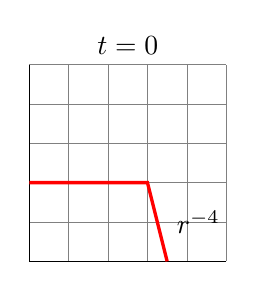
\begin{tikzpicture}
%					Tracé de la grille :
					\draw[step=.5cm,gray,very thin] (0,0) grid (2.5,2.5);
%					Tracé des axes :
					\draw (0,0) -- (0,2.5);
					\draw (0,0) -- (2.5,0);
%					Tracé du graphe :
					\draw[red,very thick] (0,1.0) -- (1.5,1.0) -- (1.75,0);
%					\draw[red,very thick] (1.5,1.0) -- (1.75,0);
					\draw (1.75,0.5) node[right]{$r^{-4}$};
					\draw (1.25,2.5) node[above]{$t = 0$};
				\end{tikzpicture}
			\end{center}
		\end{minipage}\hfill
		\begin{minipage}[b]{0.20\linewidth}
			\begin{center}
				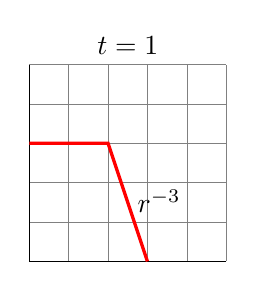
\begin{tikzpicture}
%					Tracé de la grille :
					\draw[step=.5cm,gray,very thin] (0,0) grid (2.5,2.5);
%					Tracé des axes :
					\draw (0,0) -- (0,2.5);
					\draw (0,0) -- (2.5,0);
%					Tracé du graphe :
					\draw[red,very thick] (0,1.5) -- (1,1.5) -- (1.5,0);
%					\draw[red,very thick] (1,1.5) -- (1.5,0);
					\draw (1.25,0.5) node[above right]{$r^{-3}$};
					\draw (1.25,2.5) node[above]{$t = 1$};
				\end{tikzpicture}
			\end{center}
		\end{minipage}\hfill
		\begin{minipage}[b]{0.24\linewidth}
			\begin{center}
				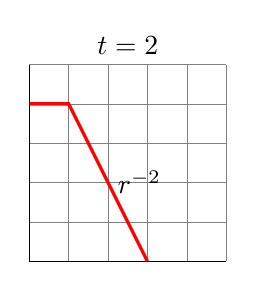
\begin{tikzpicture}
%					Tracé de la grille :
					\draw[step=.5cm,gray,very thin] (0,0) grid (2.5,2.5);
%					Tracé des axes :
					\draw (0,0) -- (0,2.5);
					\draw (0,0) -- (2.5,0);
%					Tracé du graphe :
					\draw[red,very thick] (0,2) -- (0.5,2) -- (1.5,0);
%					\draw[red,very thick] (0.5,2) -- (1.5,0);
					\draw (1,1) node[right]{$r^{-2}$};
					\draw (1.25,2.5) node[above]{$t = 2$};
				\end{tikzpicture}
			\end{center}
		\end{minipage}\hfill
		\begin{minipage}[b]{0.20\linewidth}
			\begin{center}
				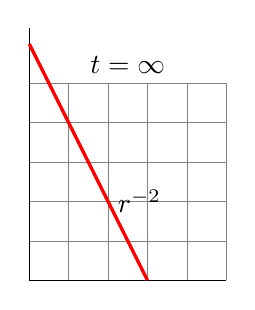
\begin{tikzpicture}
%					Tracé de la grille :
					\draw[step=.5cm,gray,very thin] (0,0) grid (2.5,2.5);
%					Tracé des axes :
					\draw (0,0) -- (0,3.2);
					\draw (0,0) -- (2.5,0);
%					Tracé du graphe :
					\draw[red,very thick] (0,3) -- (1.5,0);
					\draw (1,1) node[right]{$r^{-2}$};
					\draw (1.25,2.5) node[above]{$t = \infty$};
				\end{tikzpicture}
			\end{center}
		\end{minipage}
		\caption{Schéma d'évolution dynamique d'un amas globulaire.\label{schema-effondrement}}
	\end{figure}



Pour expliquer cette évolution, nous devons trouver quels phénomènes, de dynamique gravitationnelle, pourraient diluer le halo et concentrer de la matière au centre de l'amas. Le phénomène qui vient le plus naturellement à l'esprit est la perte d'étoiles, pouvant s'effectuer par 2 scénarios :
\begin{enumerate}
	\item des collisions internes qui éjectent des étoiles de l'amas, permettant ainsi au cœur de s'effondrer en essayant de compenser cette perte d'énergie.
	\item des interactions avec un autre objet massif qui va retirer par effet de marée des étoiles à l'amas, causant l'effondrement de son cœur.
\end{enumerate}
C'est ce deuxième scénario que nous allons tenter d'étudier.
















%Si la température cinétique du halo augmente, celle du
%cœur va changer pour s'adapter. La capacité calorifique à volume
%constant est négative pour le cœur (~et pour tout système
%auto gravitant~) :
%\begin{align*}
%	E_p &= -2E_c & \text{(~Viriel~)} \\
%	\Rightarrow E &= E_p + E_c = -E_c \\
%	\intertext{or}
%	E_c &\varpropto T \Rightarrow E\varpropto -T \\
%	\intertext{donc}
%	\Rightarrow C_v &= \frac{\partial E}{\partial T} < 0
%\end{align*}
%Cela implique que notre système ne peut que prendre de l'énergie.

%Si la température du cœur augmente, la vitesse de rotation des
%étoiles va augmenter (~$E_c\varpropto T\varpropto v$~), et donc
%leur demi grand axe va diminuer~\footnote{rappel : $v^2 =
%K\left(\frac{2}{r} - \frac{1}{a}\right)$ avec $K = G\left(M+m\right)$
%pour des interactions à deux corps}.
%En conséquent la densité au centre du cœur augmente, augmentant
%ainsi le contraste de densité. Si la température augmente
%suffisamment, le contraste de densité du halo va dépasser la
%valeur critique $\R_c^H$ (~l'énergie est fixé, seul la
%température change, nous utilisons donc la description micro
%canonique~). Le cœur va alors devenir instable.


%	L'interprétation semble simple ici : par exemple : quand les étoiles
%	ont des vitesses de rotation élevées la sphère a une température élevée,
%	et donc sa capacité calorifique à volume constant, $C_v = \frac{\partial H}{\partial T} < 0$
%	(~négatif car $E_p=-2E_c\Rightarrow H=E_c+E_p=-E_c\varpropto-T$~),
%	tend vers $0$ : elle ne peut plus acquérir d'énergie.
%	Si on dépasse la limite de température, elle va devoir se \og~réorganiser~\fg pour
%	rester à l'équilibre et donc pour retourner à un contraste de densité $\R < \R^\beta_c$.
%	Le raisonnement est le même pour la limite en énergie.
